\subsection*{Flow-Aligned V-JEPA Video Handling}
\paragraph{Hypothesis tested.}
The video V-JEPA DTA/RAFT experiment tests whether past--target and target--future tubelets contain complementary temporal and appearance information that represents the target scene better than a single-image feature alone.

\paragraph{Approach.}
The four-frame clip $[I_{t-1},I_t,I_t,I_{t+1}]$ produces two V-JEPA~2.1 tubelet positions. DTA learns whether the past--target or target--future tubelet is more useful at each location. RAFT attempts to align these observations before they are combined. Specifically, unaligned DTA aggregates tokens at the same patch coordinate, although UAV motion can move a physical surface between coordinates. The alignment diagnostic therefore uses frozen RAFT target-to-neighbor flow \cite{teed2020raft}, rejects out-of-view and forward--backward-inconsistent correspondences \cite{meister2018unflow}, averages valid frame flows within each two-frame tubelet, and backward-warps the contextual tubelet features into target coordinates before validity-masked DTA. The proposed two-row visualization should retain the original four-frame/tubelet-PCA sequence, then show RAFT flow, validity masks, unaligned versus aligned PCA, DTA attention, and predicted depth.

RAFT alignment is used immediately before DTA in two specific ways:
\begin{enumerate}
    \item it spatially warps the two V-JEPA tubelet feature grids; and
    \item it supplies validity masks that tell DTA which warped tokens are reliable.
\end{enumerate}

For the illustrated OccuFly clip, DTA did not collapse to one tubelet; it used both temporal directions differently across the image.

In the target-frame coordinate system, DTA produces a $24\times24$ fused feature map. At each cell, it learns how much to use from the aligned past--target and target--future tubelet features to minimize the target image's depth-prediction loss. DTA does not directly know which feature represents the ``actual depth.'' It learns this preference indirectly through backpropagation from the target-depth ground truth. The fused $24\times24$ features are then decoded into the full-resolution target depth map.

\begin{figure}[t]
    \centering
    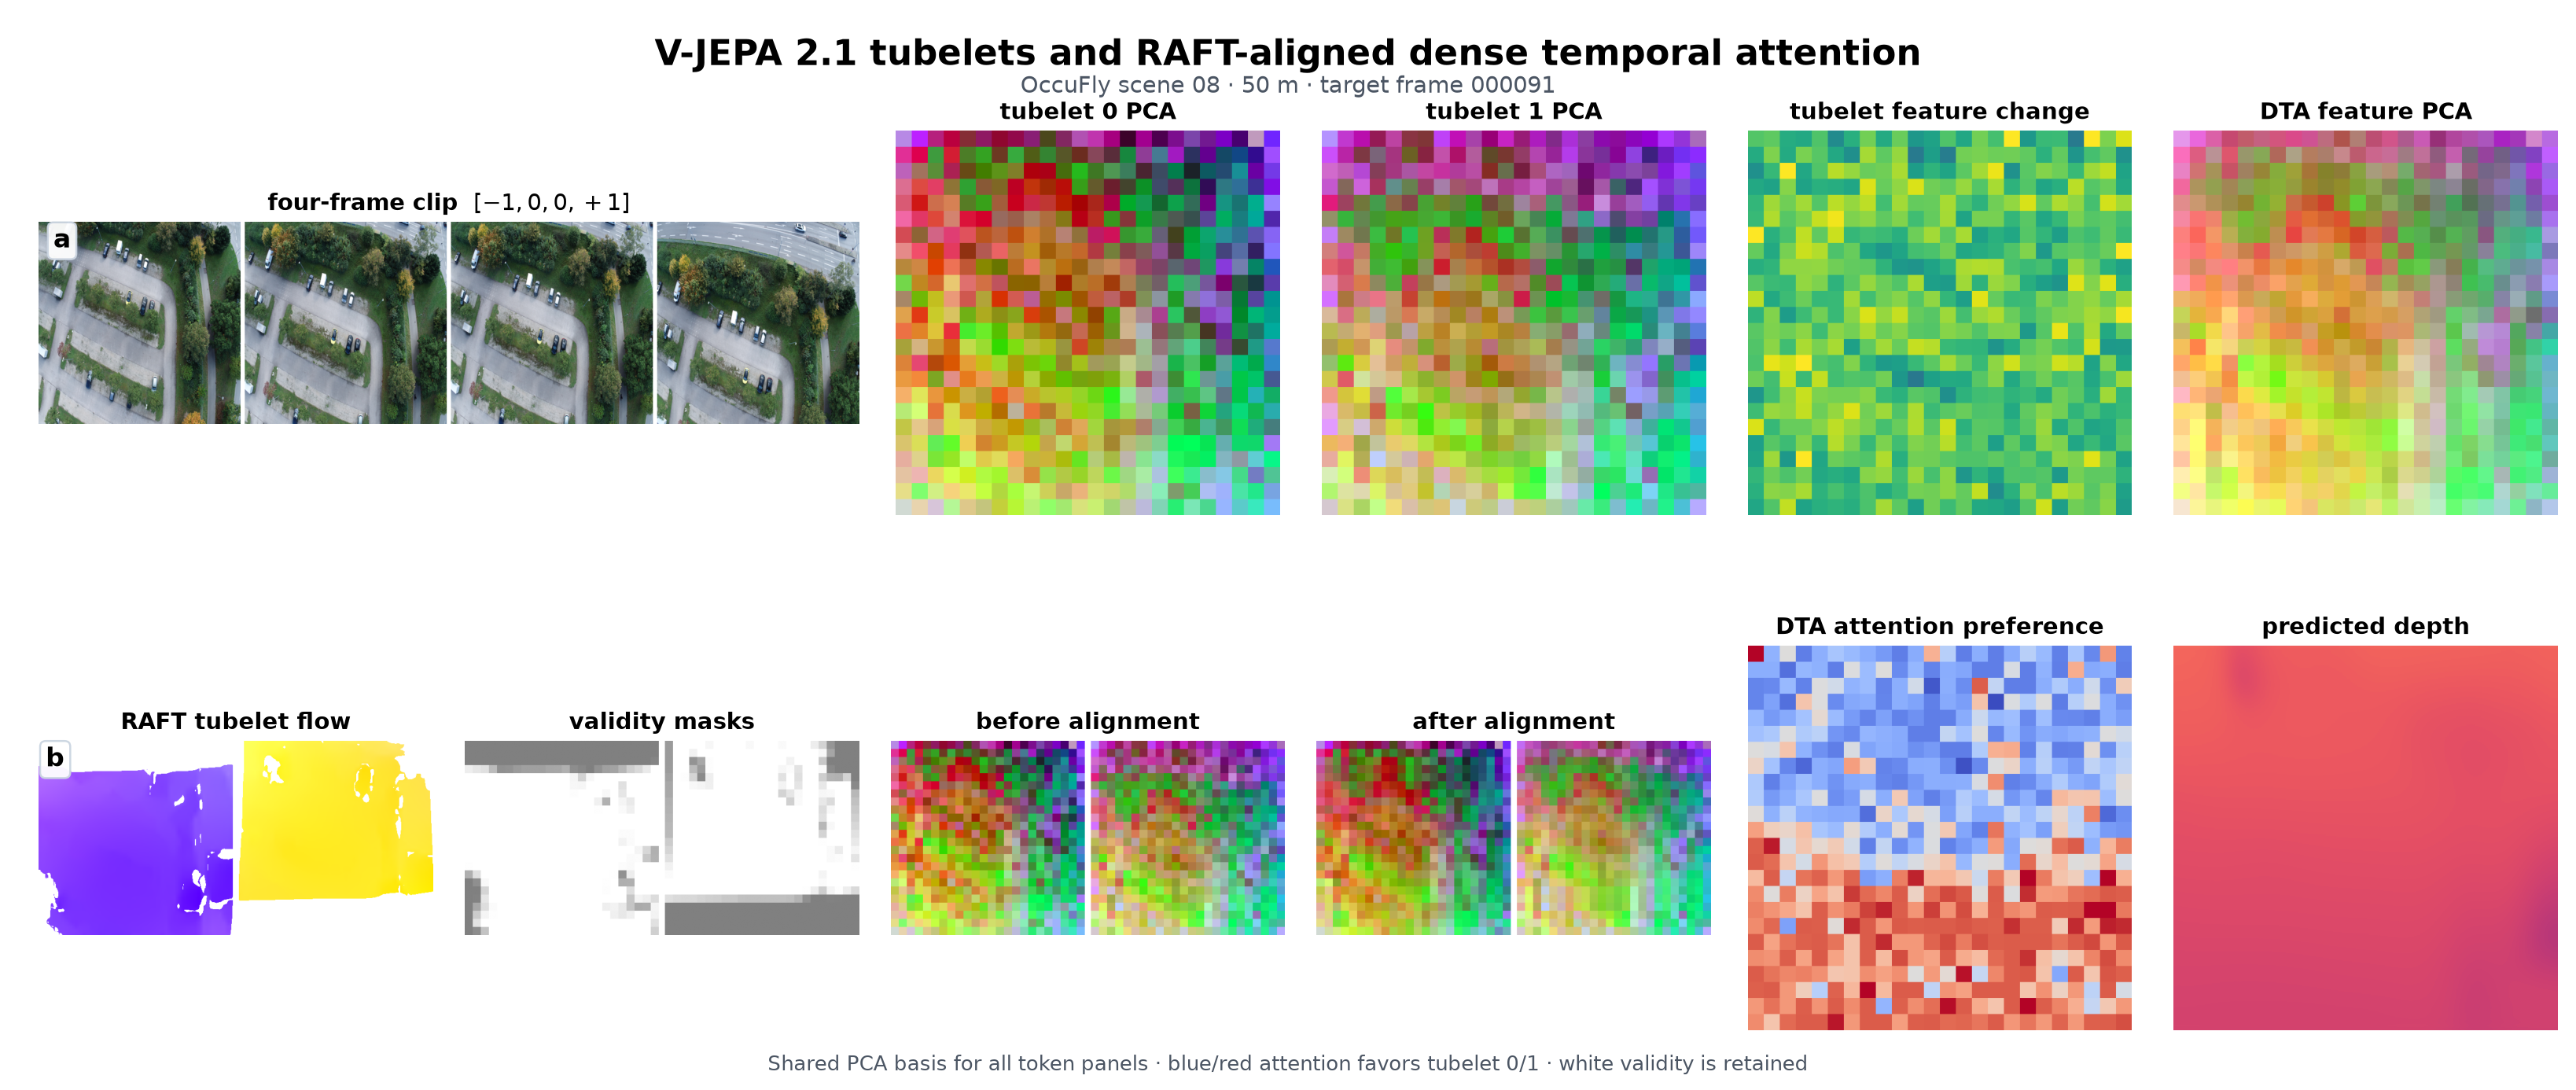
\includegraphics[width=\linewidth]{content/images/vjepa_video_raft_figure3_extension_preview.png}
    \caption{Checkpoint-derived V-JEPA/RAFT diagnostic for the illustrated OccuFly clip. In the DTA attention-preference panel, blue favors the past--target tubelet, red favors the target--future tubelet, and white indicates approximately equal average attention across the eight heads. The spatial pattern demonstrates use of both temporal directions, but does not by itself establish improved depth accuracy.}
    \label{fig:notes_vjepa_raft_dta_preference}
\end{figure}

\paragraph{What video could add.}
Compared with a single target image, adjacent frames can provide repeated observations, motion parallax, changing visibility at occlusion boundaries, and temporally complementary features. DTA can select between the two tubelets locally, while RAFT reduces the coordinate mismatch caused by camera or scene motion before fusion.

\paragraph{Why this may not beat monocular training.}
Optical flow supplies two-dimensional correspondence rather than metric geometry; it can be unreliable in occluded, blurred, repetitive, or textureless regions, and post-encoding warping cannot reverse information already mixed within a V-JEPA tubelet. A strong monocular model can also exploit appearance together with camera intrinsics and altitude without incurring flow errors or additional video computation. Empirically, video DTA improves over the weakest RGB linear readout in $\delta_1$ ($0.701$ versus $0.651$) and RMSE ($7.055$ versus $7.808$\,m), but not AbsRel ($0.191$ versus $0.189$). Thus, V-JEPA video features provide complementary temporal information, but the current DTA/RAFT interface does not yet convert that information into a consistent advantage over camera-conditioned monocular depth estimation.

\paragraph{Limitations and literature context.}
Flow warping with occlusion handling is established for temporal depth consistency \cite{li2021temporalconsistency}, while pose/depth-based state warping provides a more geometric alternative when calibration and metric structure are available \cite{duzceker2021deepvideomvs}. The present RAFT path is only a post-encoding approximation: optical flow is not metric geometry, can fail under occlusion, motion blur, repetitive or textureless aerial regions, and domain shift, and cannot undo V-JEPA's two-frame tubelet mixing. Recent video-depth work likewise notes the limitations and cost of flow-based constraints and instead adopts a flow-free temporal-gradient objective \cite{chen2025videodepthanything}. Aligned-versus-unaligned claims therefore require matched evaluation and reported validity coverage.
